\chapter{Experimental Results and Comparisons}\label{ch:results}

Sections~\ref{sec:res-chrononet}--\ref{sec:res-types}: development on the 96 training patients
(patient-wise cross-validation). Sections~\ref{sec:res-test}--\ref{sec:res-hw}: the single evaluation on the 29
held-out test patients, after the design was frozen.

\section{Reproduction of the Published Baseline}\label{sec:res-chrononet}

\begin{figure}[H]
\centering
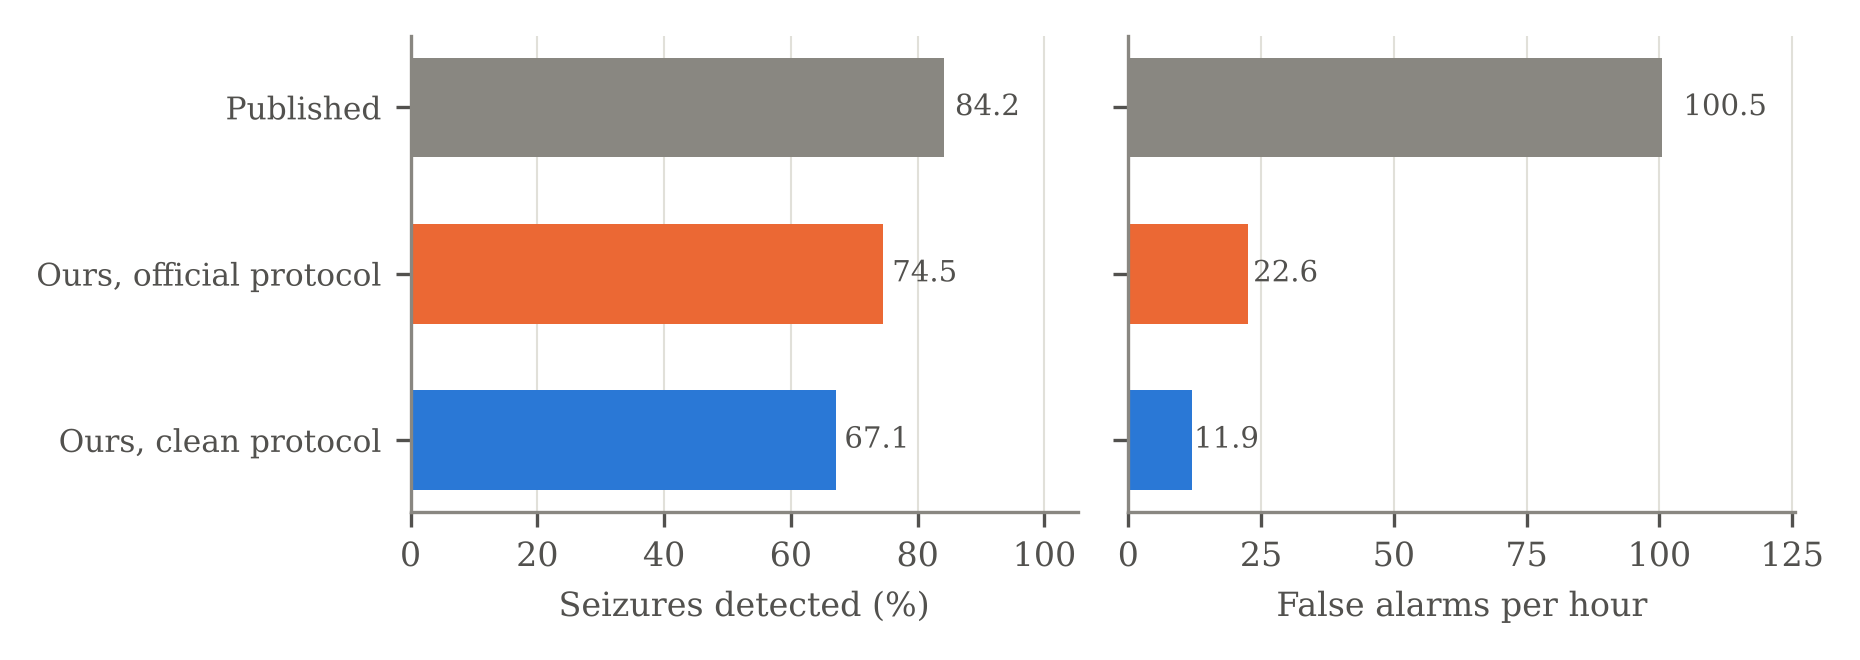
\includegraphics[width=0.9\textwidth]{figures/chrononet_repro.png}
\caption{ChronoNet on the 29 test patients: published and reproduced (the paper's metrics).}\label{fig:chrononet}
\end{figure}

\begin{itemize}
\item \textbf{Partly reproduced}: 74.5\,\% of seizures detected against 84.2\,\% published, with 22.6 instead of 100.5
  false alarms per hour (Figure~\ref{fig:chrononet}); the per-recording AUPR matches (0.109 vs 0.104).
\item \textbf{Test-set leak}: the released code picks its training epoch on the test patients. Our \textbf{clean} run
  (last epoch, no test information: 67.1\,\%, 11.9 false alarms/h) is the reference for the final comparison.
\end{itemize}

\section{Integer Versus Floating-Point Features}\label{sec:intfloat}

\begin{table}[H]
\centering\small
\caption{The integer front end against its floating-point twin (10 training patients).}\label{tab:intfloat}
\begin{tabular}{@{}lc@{}}
\toprule
\textbf{Check} & \textbf{Result}\\
\midrule
Median feature correlation, integer vs float & 0.9965\\
Artefact flags agreeing & 99.7\,\%\\
LightGBM AUROC, integer vs float features & 0.736 vs 0.735\\
\bottomrule
\end{tabular}
\end{table}

\section{Comparison of Model Families}\label{sec:res-families}

\begin{table}[H]
\centering\small
\caption{Five-fold cross-validation on the 96 training patients (best-F1 operating point).}\label{tab:families}
\begin{tabularx}{\textwidth}{@{}P{38mm}ccccL@{}}
\toprule
\textbf{Model} & \textbf{AUROC} & \textbf{Event-F1} & \textbf{FA / 24 h} & \textbf{Sens.\ at $\le$1 FA/h} & \textbf{Estimated cost}\\
\midrule
LightGBM & 0.870 & 0.292 & 3.6 & 0.594 & $\approx$30.6k LUTs\\
CatBoost & 0.863 & 0.286 & 3.0 & 0.618 & $\approx$27.7k LUTs\\
XGBoost & 0.867 & 0.277 & 3.4 & 0.603 & $\approx$47.9k LUTs\\
TreeLUT & 0.857 & 0.266 & 4.2 & 0.619 & $\approx$6.4k LUTs\\
\textbf{DWN + distillation (final)} & 0.851 & \textbf{0.229} & \textbf{0.9} & 0.597 & \textbf{$\approx$870 LUTs}\\
DWN base & 0.840 & 0.211 & 2.4 & 0.581 & $\approx$960 LUTs\\
Random forest & 0.852 & 0.198 & 0.5 & 0.536 & $\approx$323k LUTs\\
Logic-gate network & 0.843 & 0.171 & 4.9 & 0.540 & $\approx$7.5k LUTs\\
INT8 MLP & 0.830 & 0.147 & 7.8 & 0.520 & 9,600 multiplications\\
Logistic regression & 0.806 & 0.105 & 8.8 & 0.409 & 117 multiplications\\
\bottomrule
\end{tabularx}
\end{table}

\begin{figure}[H]
\centering
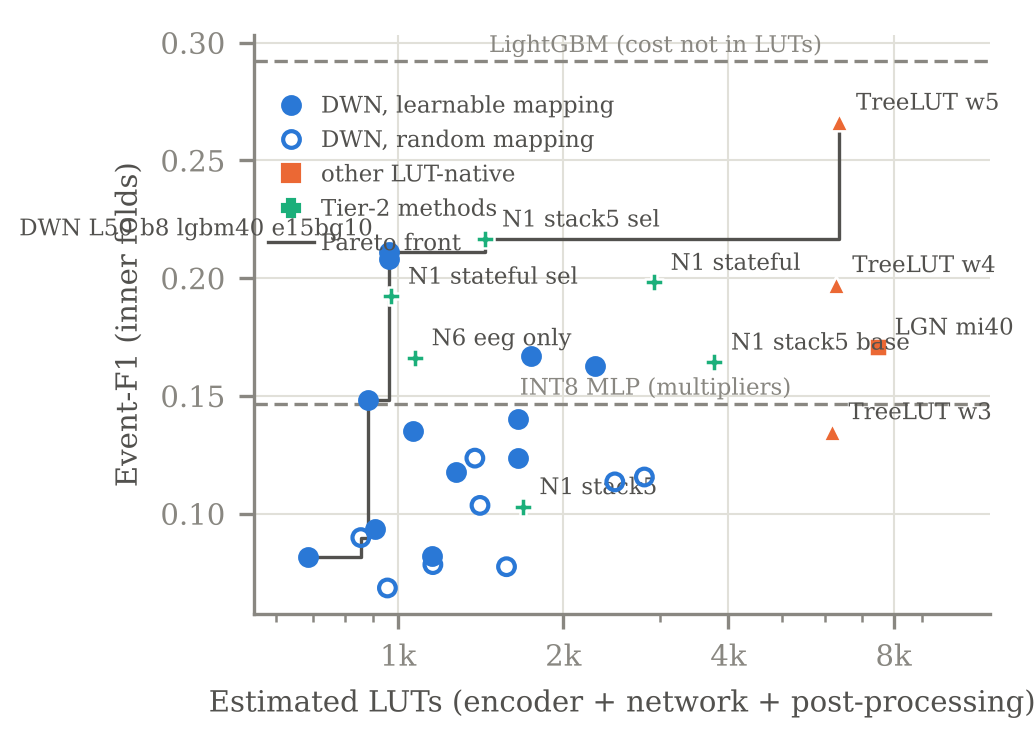
\includegraphics[width=0.68\textwidth]{figures/pareto_inner_cv.png}
\caption{Event-F1 against estimated LUTs for every LUT-native run (training folds), with the Pareto front.}\label{fig:pareto}
\end{figure}

\paragraph{Findings.} The DWN is 7--8$\times$ smaller than the other LUT models and beats the INT8 MLP on every metric
(Table~\ref{tab:families}). Larger networks (up to 2,000 LUTs), 16 thresholds, two layers and other temperatures gave no
significant gain (Figure~\ref{fig:pareto}); 4-input LUTs and 4 thresholds were clearly worse.

\section{What Improved the Network}\label{sec:res-ext}

\begin{figure}[H]
\centering
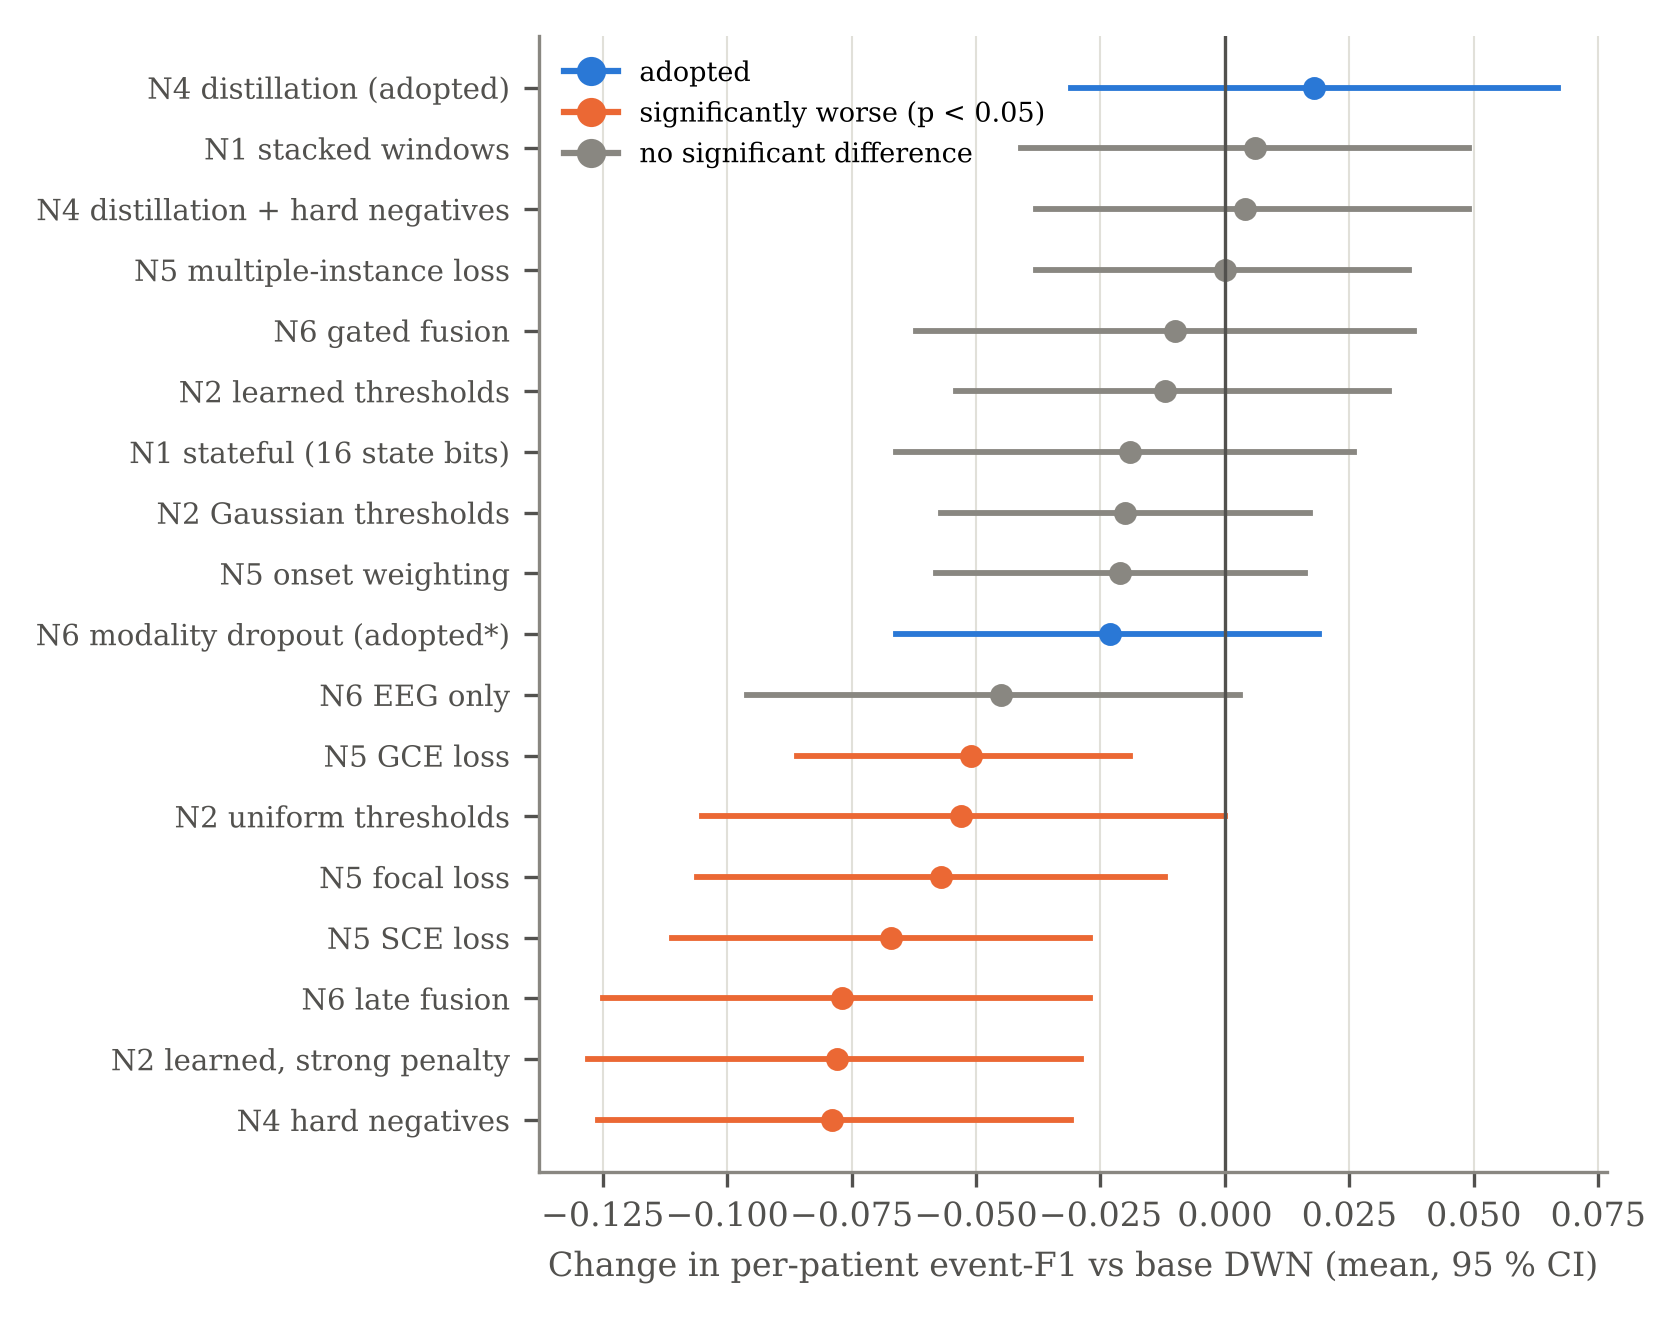
\includegraphics[width=0.85\textwidth]{figures/ablation.png}
\caption{Every extension against the base DWN: mean change in per-patient event-F1 with 95\,\% interval. *Modality
dropout was adopted for its robustness to missing sensors (Section~\ref{sec:res-missing}).}\label{fig:ablation}
\end{figure}

\begin{table}[H]
\centering\small
\caption{The changes that passed the significance test.}\label{tab:adopted}
\begin{tabularx}{\textwidth}{@{}P{42mm}LP{38mm}@{}}
\toprule
\textbf{Change} & \textbf{Evidence (training patients)} & \textbf{How it was found}\\
\midrule
Feature selection by LightGBM importance & event-F1 0.148 $\to$ 0.208 ($p = 0.047$); false alarms 7.0 $\to$ 2.3/day & N7 showed the network ignored heart rate\\
Distillation from LightGBM (\textbf{final}) & false alarms 2.4 $\to$ 0.9/day ($p = 3\times10^{-7}$); event-F1 0.229 vs 0.211 & N4\\
Modality dropout (variant) & without ECG: event-F1 0.092 $\to$ 0.172 ($p = 0.005$) & N6\\
\bottomrule
\end{tabularx}
\end{table}

\begin{figure}[H]
\centering
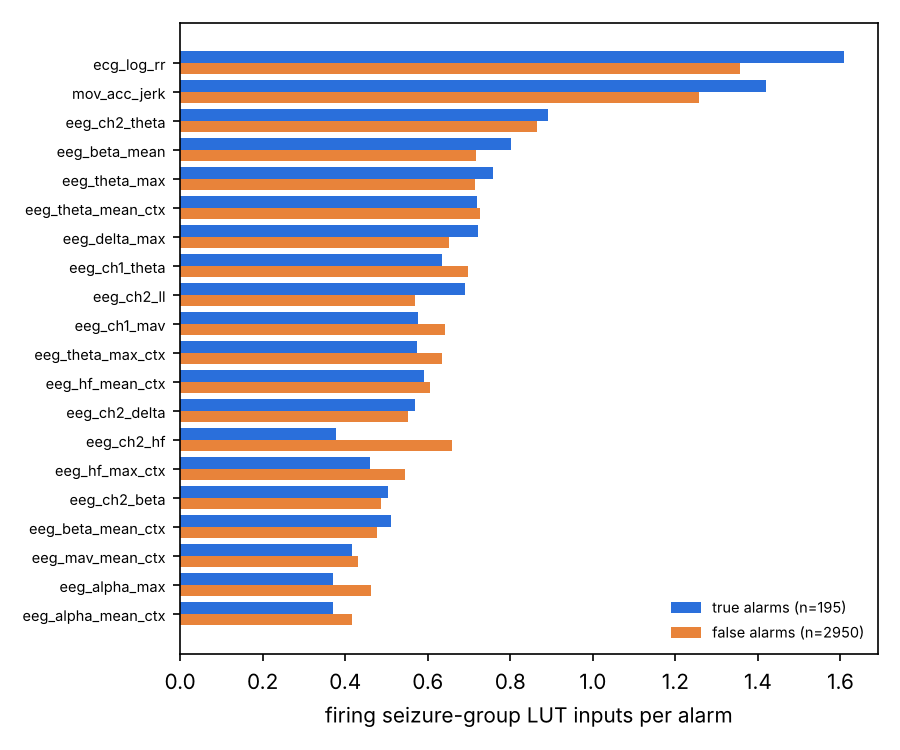
\includegraphics[width=0.55\textwidth]{figures/n7_feature_usage.png}
\caption{N7: inputs read by the firing seizure LUTs during true and false alarms (first, mutual-information network):
false alarms look like seizures to it.}\label{fig:n7}
\end{figure}

\section{Missing Sensors}\label{sec:res-missing}

\begin{figure}[H]
\centering
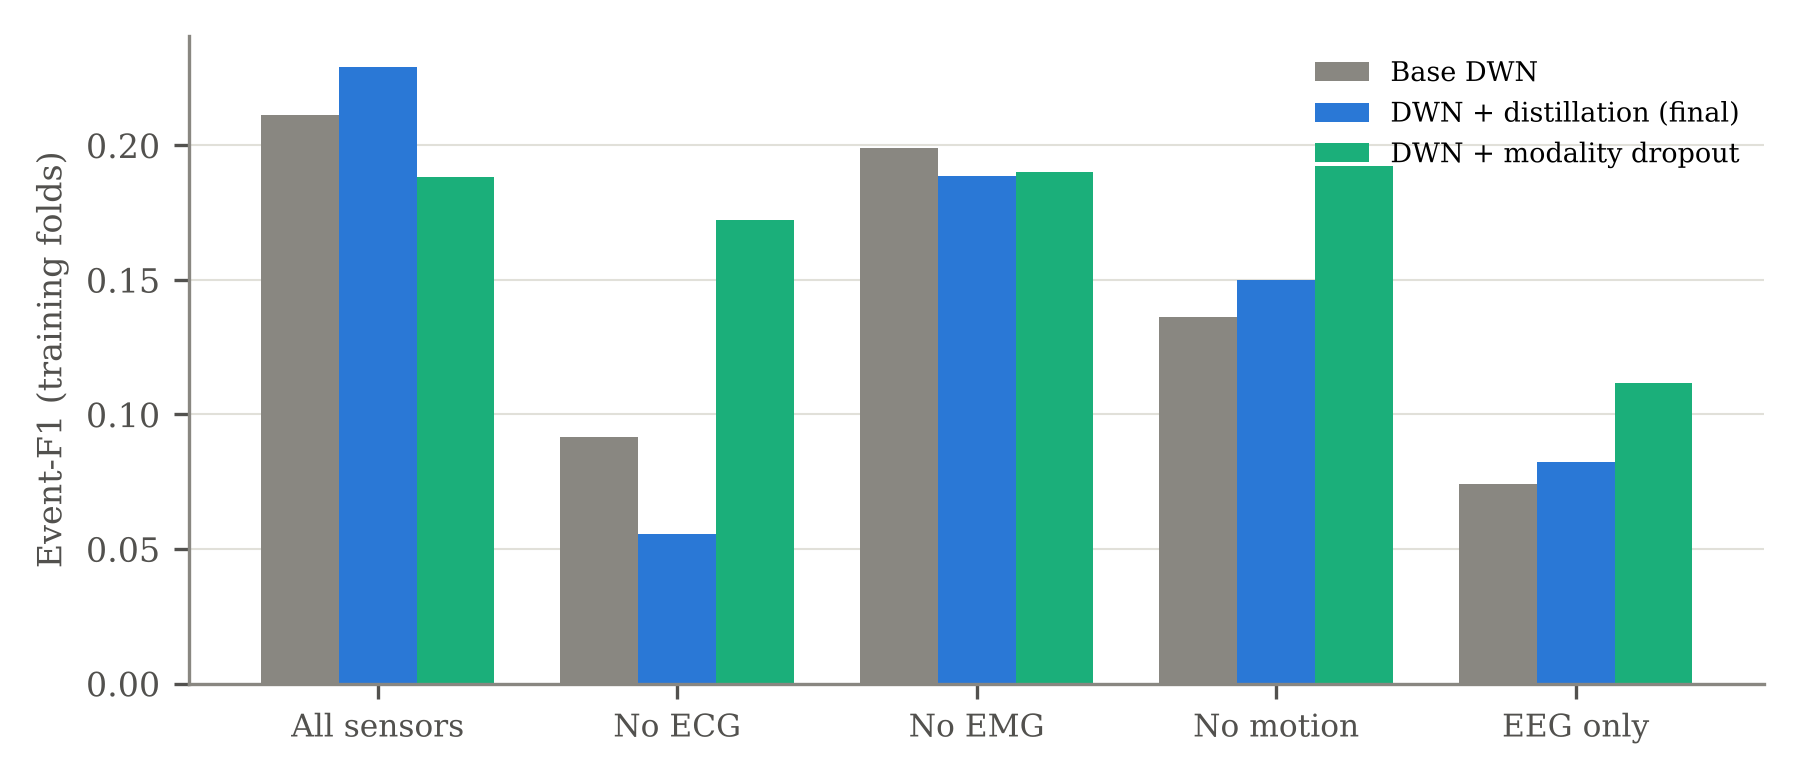
\includegraphics[width=0.85\textwidth]{figures/missing_sensors.png}
\caption{Event-F1 with sensors removed at test time (training folds). Distillation is the most accurate with all
sensors; modality dropout keeps working without ECG or motion.}\label{fig:missing}
\end{figure}

\section{Seizure Types}\label{sec:res-types}

\begin{figure}[H]
\centering
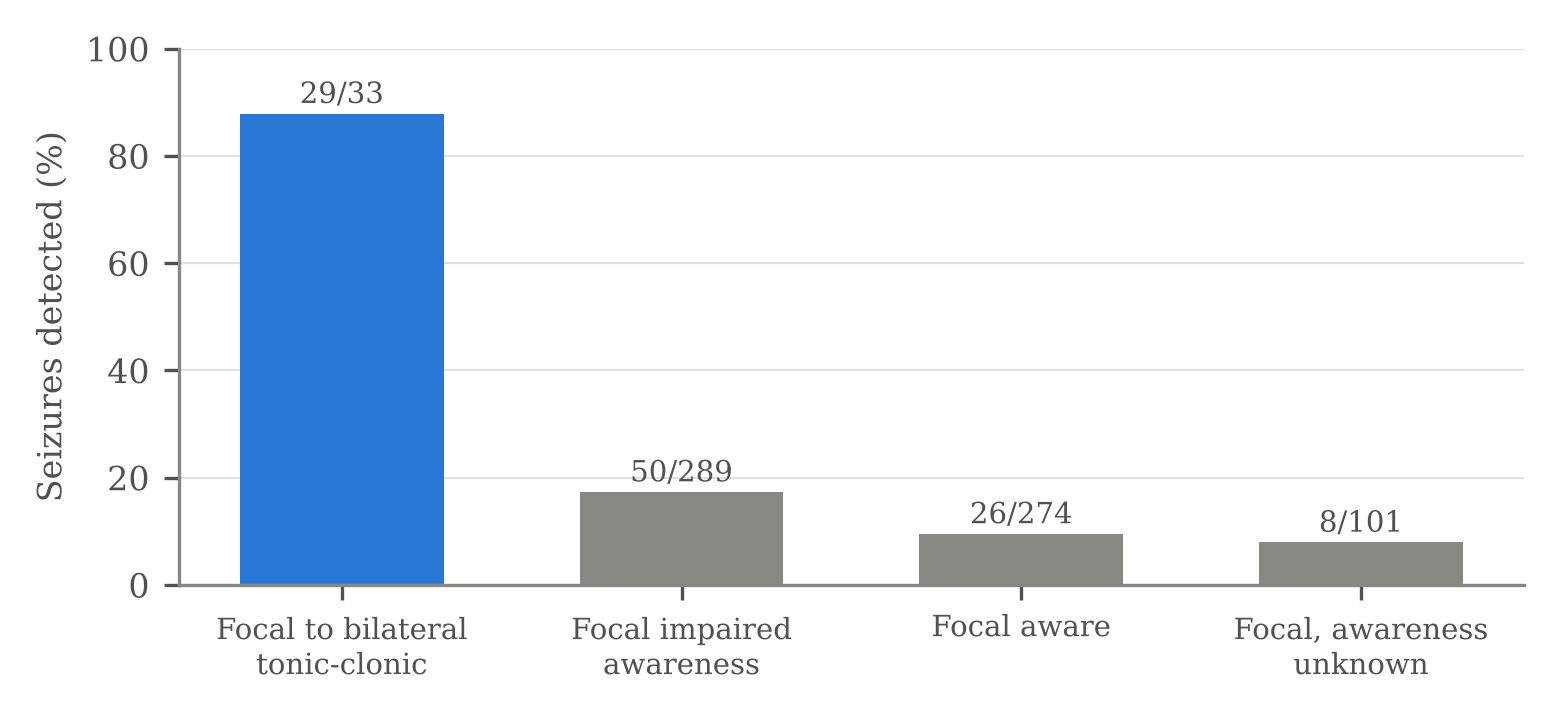
\includegraphics[width=0.65\textwidth]{figures/seizure_types.png}
\caption{Seizures detected by type (base DWN, training folds): tonic-clonic seizures are caught, focal seizures rarely.}\label{fig:types}
\end{figure}

\section{Final Evaluation on the Held-Out Test Patients}\label{sec:res-test}

\begin{figure}[H]
\centering
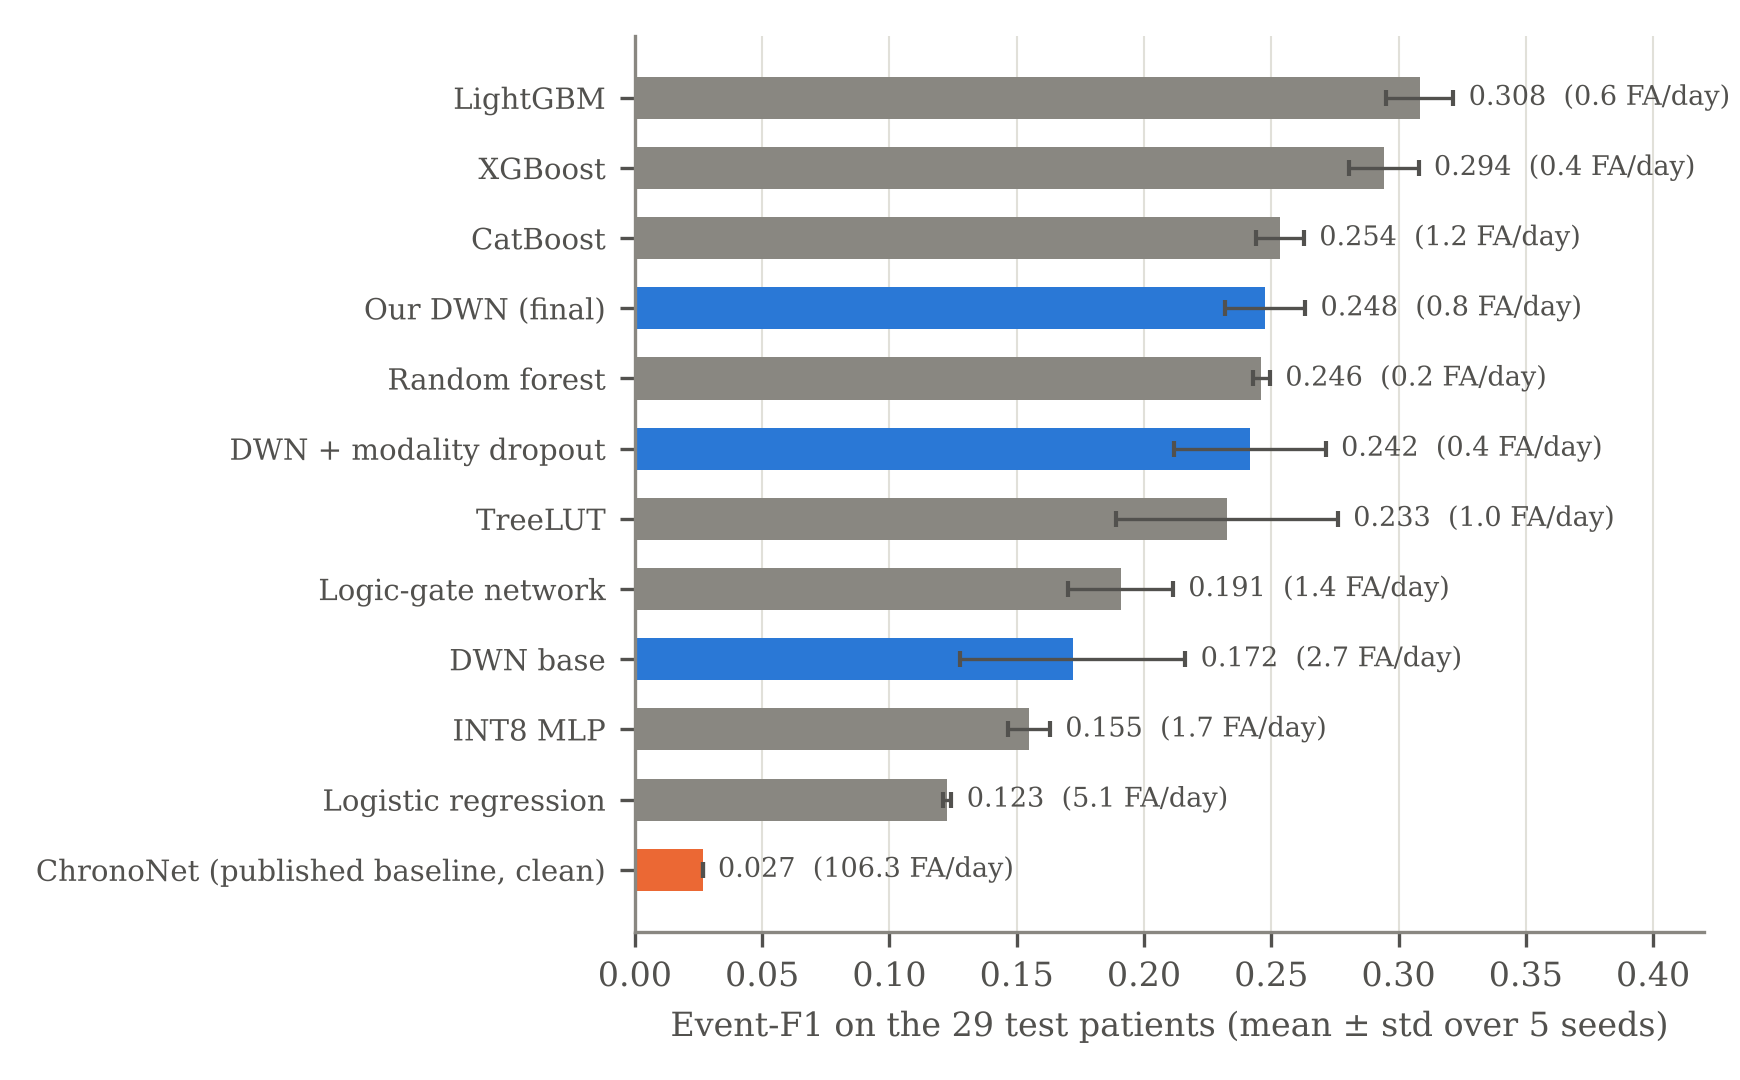
\includegraphics[width=0.85\textwidth]{figures/test_f1.png}
\caption{Event-F1 on the 29 test patients (mean $\pm$ std over 5 seeds) and false alarms per day.}\label{fig:testf1}
\end{figure}

\begin{figure}[H]
\centering
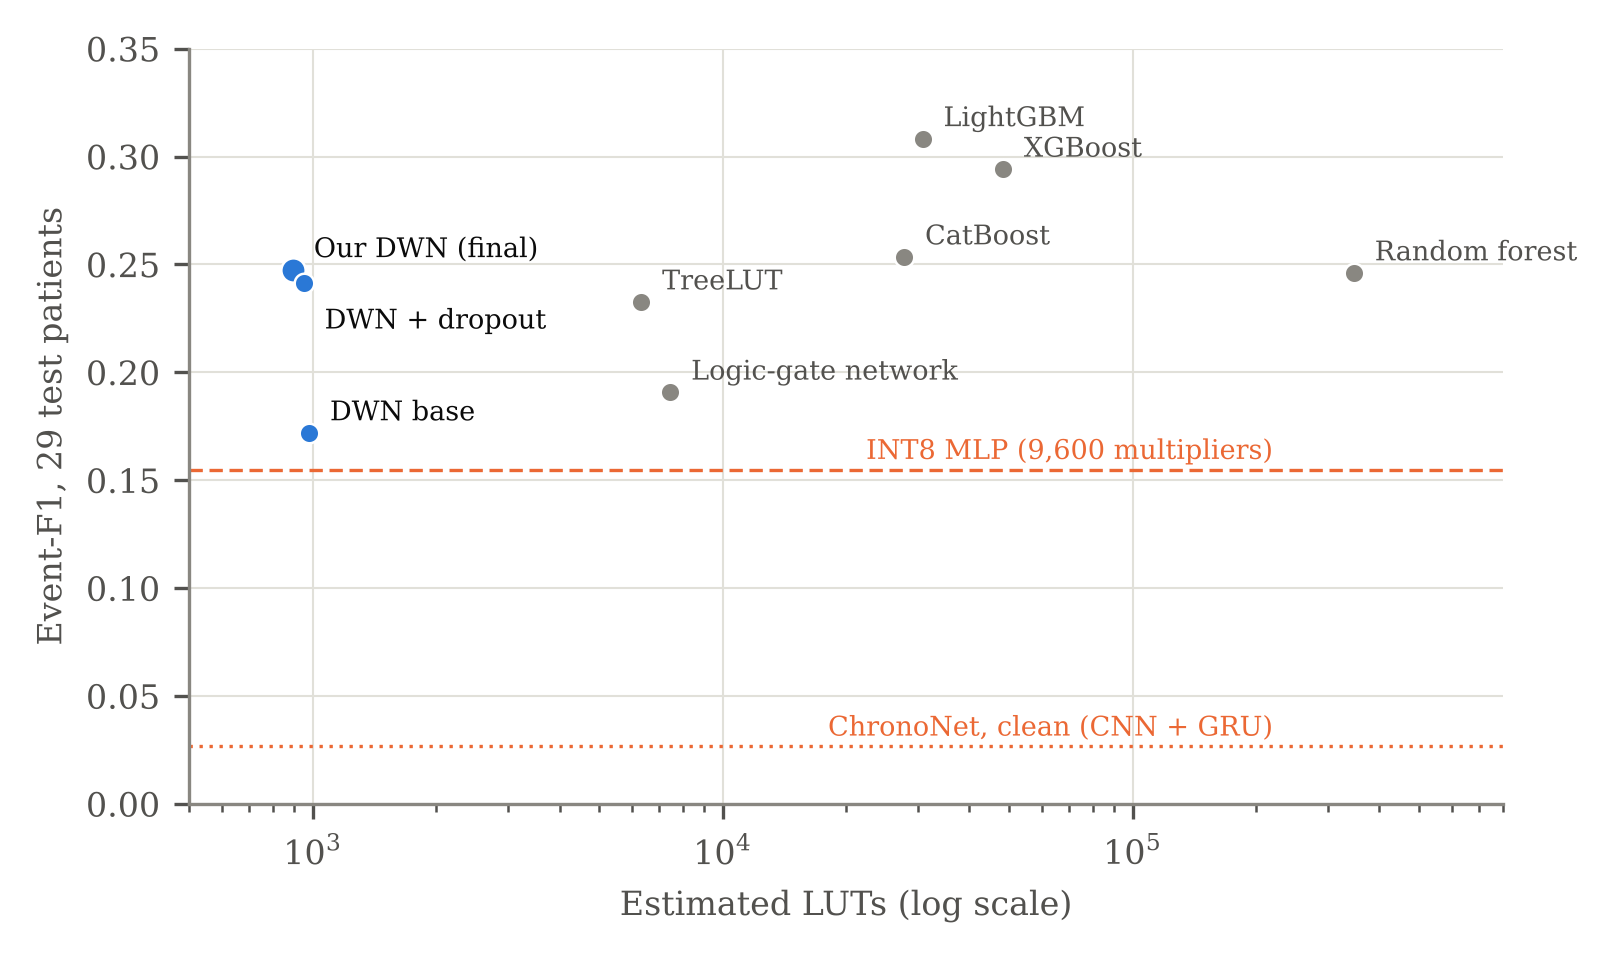
\includegraphics[width=0.8\textwidth]{figures/test_f1_vs_luts.png}
\caption{Accuracy against hardware cost on the test patients: the LUT networks reach tree-ensemble accuracy at a
fraction of the LUTs.}\label{fig:testluts}
\end{figure}

\begin{table}[H]
\centering\small
\caption[Final DWN against the main references on the 29 test patients.]{Final DWN against the main references on the 29 test patients ($p$: paired Wilcoxon on per-patient event-F1).}\label{tab:test}
\begin{tabularx}{\textwidth}{@{}P{40mm}cccL@{}}
\toprule
\textbf{Model} & \textbf{Event-F1} & \textbf{FA / 24 h} & \textbf{$p$ vs ChronoNet} & \textbf{Estimated cost}\\
\midrule
\textbf{DWN + distillation (final)} & \textbf{0.248 $\pm$ 0.016} & \textbf{0.8} & 0.027 & \textbf{$\approx$900 LUTs}\\
LightGBM & 0.308 $\pm$ 0.013 & 0.6 & 0.027 & $\approx$30.8k LUTs\\
CatBoost & 0.254 $\pm$ 0.009 & 1.2 & 0.031 & $\approx$27.7k LUTs\\
Random forest & 0.246 $\pm$ 0.003 & 0.2 & 0.27 & $\approx$347k LUTs\\
TreeLUT & 0.233 $\pm$ 0.044 & 1.0 & 0.016 & $\approx$6.3k LUTs\\
Logic-gate network & 0.191 $\pm$ 0.021 & 1.4 & 0.034 & $\approx$7.5k LUTs\\
INT8 MLP & 0.155 $\pm$ 0.008 & 1.7 & 0.017 & 9,600 multiplications\\
ChronoNet (clean) & 0.027 & 106 & -- & CNN + GRU\\
\bottomrule
\end{tabularx}
\end{table}

\paragraph{Findings.} The result held on unseen patients (0.248, above the cross-validation 0.229). The final DWN scores
above TreeLUT, the logic-gate network and the INT8 MLP, is level with random forest and CatBoost at 30--390$\times$ fewer
LUTs, and is significantly better than ChronoNet; LightGBM remains ahead ($p = 0.039$). All 11 models are in
Table~\ref{tab:test-full} (Appendix~\ref{app:sources}).

\section{Comparison with the Base Paper}\label{sec:res-published}

\begin{figure}[H]
\centering
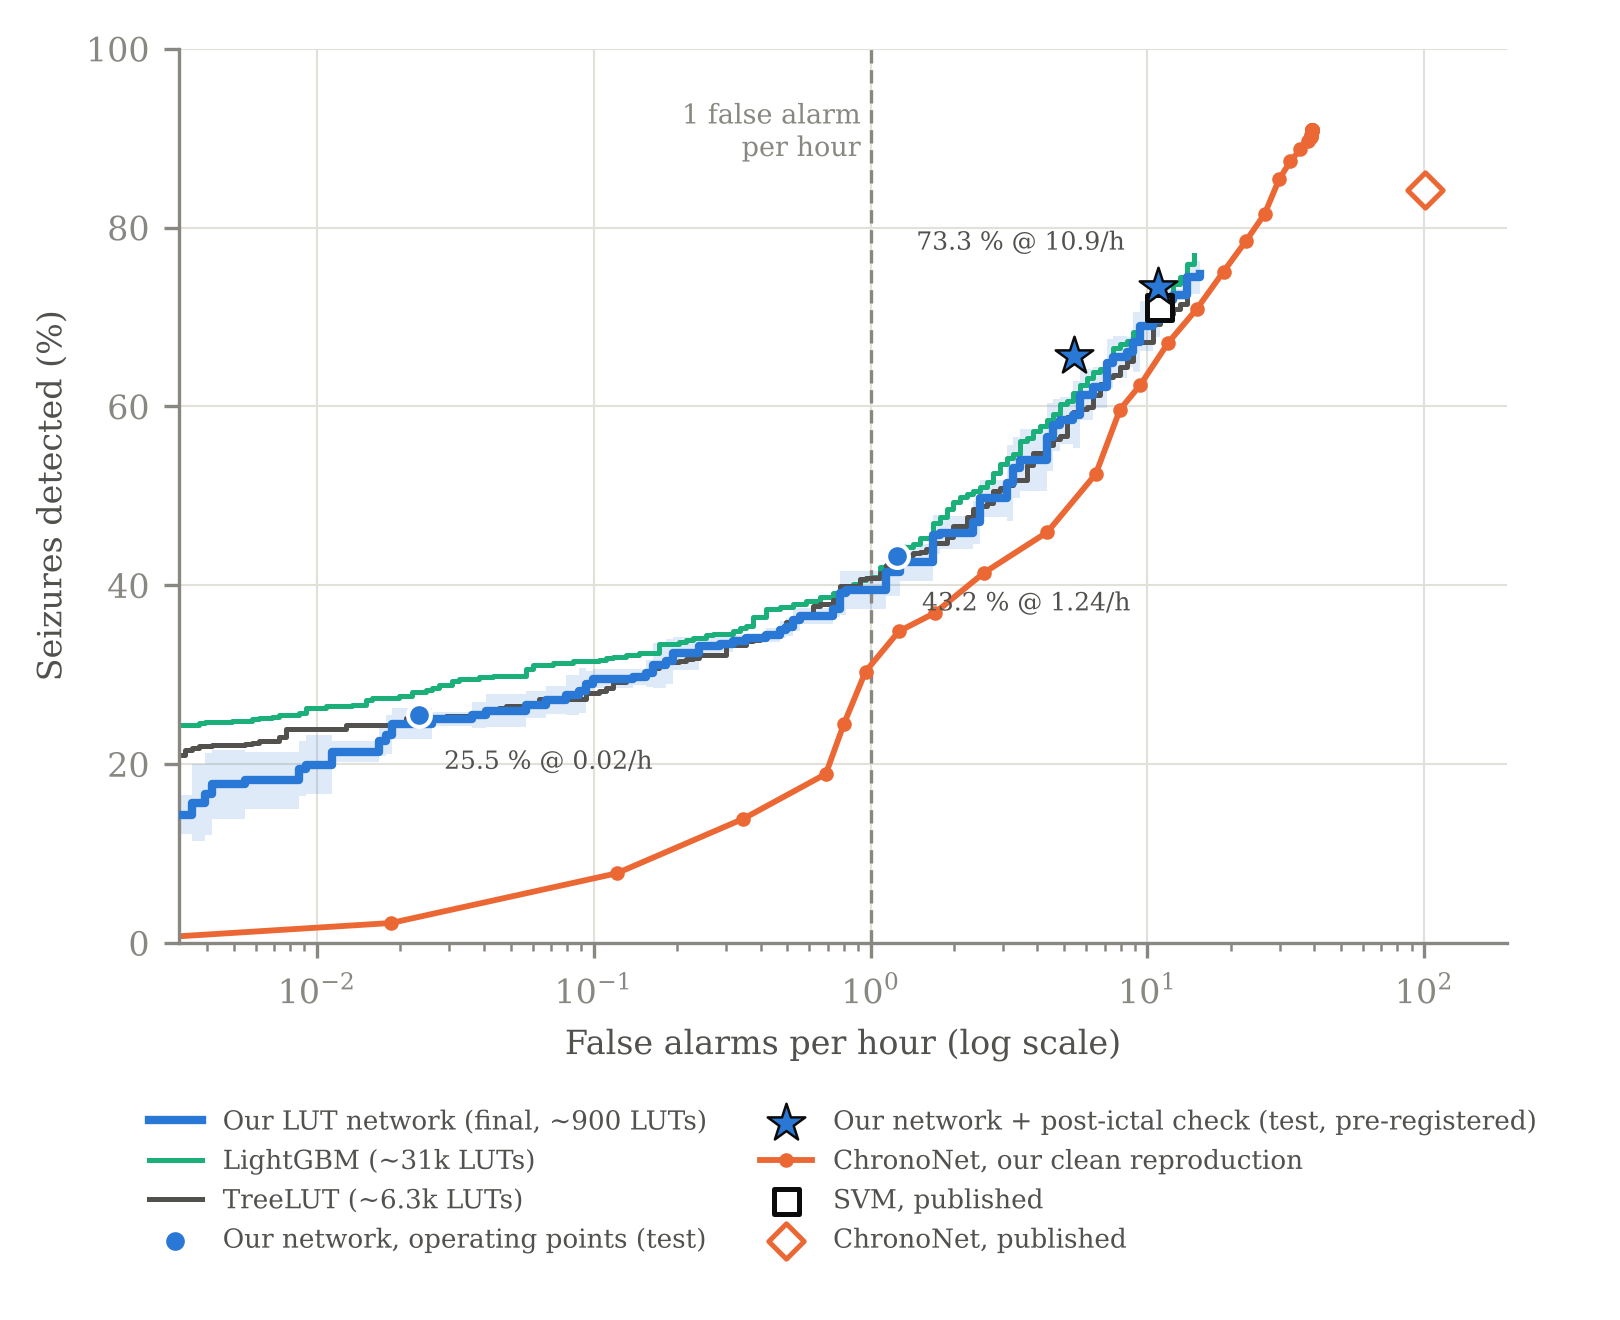
\includegraphics[width=0.85\textwidth]{figures/sens_fa_test.png}
\caption{Seizures detected against false alarms per hour on the 29 test patients (the base paper's metrics). Curves:
threshold sweeps of the frozen models (mean of 5 seeds; band: std of our network), drawn as far as every seed's sweep
reaches; dots: our two operating points, chosen on the training folds; stars: the two-stage detector
(Section~\ref{sec:res-n8}); open markers: published values.}\label{fig:sensfa}
\end{figure}

\begin{table}[H]
\centering\small
\caption{The base paper's baselines and our network on the same 29 test patients (the paper's metrics).}\label{tab:published}
\begin{tabularx}{\textwidth}{@{}P{70mm}ccL@{}}
\toprule
\textbf{Model} & \textbf{Detected} & \textbf{FA / h} & \textbf{AUROC}\\
\midrule
SVM, published \cite{bhagubai2025seizeit2} & 71.1\,\% & 11.0 & 0.700\\
ChronoNet, published \cite{bhagubai2025seizeit2} & 84.2\,\% & 100.5 & 0.792\\
ChronoNet, our clean reproduction & 67.1\,\% & 11.9 & 0.746\\
ChronoNet at $\approx$1.3 FA/h$^{*}$ & 34.8\,\% & 1.26 & --\\
\textbf{Our DWN, $\le$1 FA/h operating point} & \textbf{43.2\,\%} & \textbf{1.24} & \textbf{0.883}\\
\textbf{Our DWN, best-F1 operating point} & \textbf{25.5\,\%} & \textbf{0.02} & \\
\textbf{Our DWN + post-ictal check (pre-registered)$^{\dagger}$} & \textbf{73.3\,\%} & \textbf{10.9} & \\
\textbf{Same, stricter verification$^{\dagger}$} & \textbf{65.6\,\%} & \textbf{5.4} & \\
\bottomrule
\multicolumn{4}{@{}p{\textwidth}@{}}{\footnotesize $^{*}$ threshold read from ChronoNet's own test curve (favours it); at
0.02 FA/h ChronoNet detects 2.2\,\%. AUROC pooled over test windows; the published 0.792 uses an unreproduced definition.
$^{\dagger}$ Secondary analysis after the final test (Section~\ref{sec:res-n8}); 96\,s decision delay.}
\end{tabularx}
\end{table}

\paragraph{Findings.} The paper's baselines run at 11--100 false alarms per hour. At the same false-alarm rate our
network detects more seizures than ChronoNet (43.2\,\% vs 34.8\,\% at $\approx$1.25/h; 25.5\,\% vs 2.2\,\% at
$\approx$0.02/h), ranks windows better (AUROC 0.883 vs 0.746), and needs no multipliers. At the SVM's rate of 11 false
alarms per hour its curve reaches 69.7\,\% (SVM, published: 71.1\,\%), level with LightGBM (70.5\,\%) at 3\,\% of its
LUTs; this value is read from the test curve itself and is therefore optimistic.

\section{Post-Ictal Verification (Secondary Analysis)}\label{sec:res-n8}

Requested after the final test: detect more seizures than the base paper at slightly fewer false alarms. A two-stage
detector (N8) runs the final network at a sensitive threshold and confirms each alarm 96\,s later with a second LUT
network (50 LUTs) that compares the alarm with the minutes before and after it (EEG, heart rate, EMG, motion). All
settings were chosen on the training patients and committed before one evaluation on the test patients.

\begin{table}[H]
\centering\small
\caption[Two-stage detector with post-ictal verification.]{Two-stage detector: training patients (cross-validation) and test patients (5 seeds, paper's metrics).}\label{tab:n8}
\begin{tabular}{@{}lcccc@{}}
\toprule
\textbf{Detector} & \multicolumn{2}{c}{\textbf{Training (CV)}} & \multicolumn{2}{c}{\textbf{Test}}\\
 & Detected & FA/h & Detected & FA/h\\
\midrule
Final network, lower threshold & 74.2\,\% & 8.5 & 66.4 $\pm$ 2.0\,\% & 7.6\\
\textbf{+ post-ictal check ($\le$10 FA/h)} & 81.9\,\% & 9.6 & \textbf{73.3 $\pm$ 1.4\,\%} & \textbf{10.9}\\
+ post-ictal check ($\le$5 FA/h) & 72.3\,\% & 4.8 & 65.6 $\pm$ 1.0\,\% & 5.4\\
SVM, published \cite{bhagubai2025seizeit2} & -- & -- & 71.1\,\% & 11.0\\
\bottomrule
\end{tabular}
\end{table}

\paragraph{Findings.} At the SVM's false-alarm rate (10.9 vs 11.0 per hour) the LUT-native two-stage detector detects
2.2 points more seizures (all 5 seeds above 71.1\,\%; a small margin against a single published value). Verification
adds 3.6--6.5 points over the network alone at the same false-alarm rate. Costs: a 96\,s decision delay (seizure
logging, not instant alarms) and many false alarms per day, as for the paper's baselines; the low-false-alarm result of
Section~\ref{sec:res-test} remains the primary one.

\section{Hardware Handoff Check}\label{sec:res-hw}

\begin{table}[H]
\centering\small
\caption{Verilog of the final DWN against the software on 10 test recordings.}\label{tab:verilog}
\begin{tabular}{@{}ll@{}}
\toprule
\textbf{Item} & \textbf{Result}\\
\midrule
Exported & thresholds, input mapping, 50 truth tables, popcount head\\
Test vectors & raw samples, features, bits, LUT outputs, scores, alarms\\
Windows simulated (Icarus Verilog) & 431,960\\
Mismatches & \textbf{0}\\
\bottomrule
\end{tabular}
\end{table}
